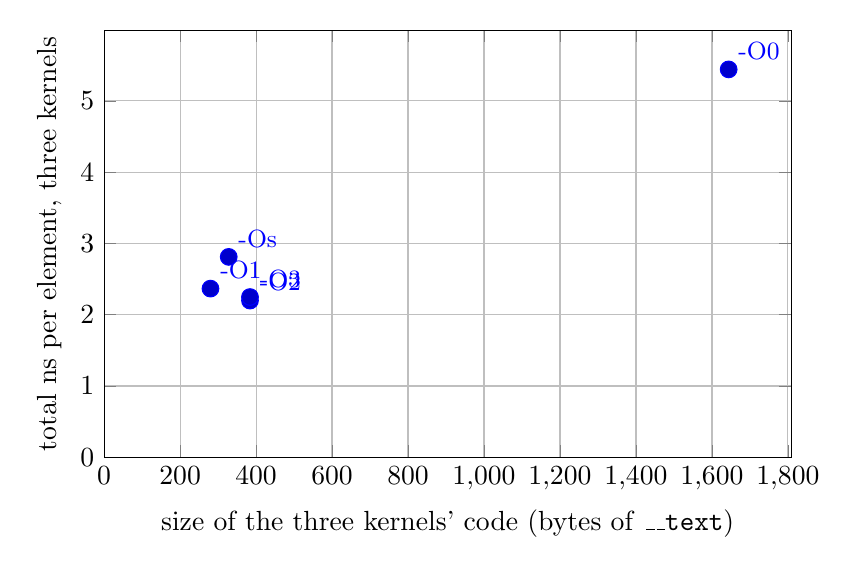
\begin{tikzpicture}
\begin{axis}[width=0.85\textwidth, height=7cm, xlabel={size of the three kernels' code (bytes of \texttt{\_\_text})}, ylabel={total ns per element, three kernels}, grid=major, xmin=0, ymin=0,
  nodes near coords, point meta=explicit symbolic, nodes near coords style={font=\small, anchor=south west}]
\addplot+[only marks, mark=*, mark size=3pt] coordinates {(1644,5.441) [-O0] (280,2.366) [-O1] (328,2.811) [-Os] (384,2.198) [-O2] (384,2.248) [-O3]};
\end{axis}
\end{tikzpicture}